\documentclass[10pt,a4paper,spanish]{report}

\usepackage[spanish]{babel}
\usepackage[utf8]{inputenc}
\usepackage{amsmath, amsthm}
\usepackage{amsfonts, amssymb, latexsym}
\usepackage{enumerate}
\usepackage[official]{eurosym}
\usepackage{graphicx}
\usepackage[usenames, dvipsnames]{color}
\usepackage{colortbl}
\usepackage{multirow}
\usepackage{fancyhdr}
\usepackage[all]{xy}
\usepackage{pgfplots}
\usepackage{algpseudocode}
\usepackage{listings}
\usepackage{titlesec}

\pgfplotsset{compat=1.5}

% a4large.sty -- fill an A4 (210mm x 297mm) page
% Note: 1 inch = 25.4 mm = 72.27 pt
%       1 pt = 3.5 mm (approx)

% vertical page layout -- one inch margin top and bottom
\topmargin      0 mm    % top margin less 1 inch
\headheight     0 mm    % height of box containing the head
\headsep       10 mm    % space between the head and the body of the page
\textheight   250 mm
\footskip      14 mm    % distance from bottom of body to bottom of foot

% horizontal page layout -- one inch margin each side
%\oddsidemargin    0   mm    % inner margin less one inch on odd pages
%\evensidemargin   0   mm    % inner margin less one inch on even pages
%\textwidth      159.2 mm    % normal width of text on page

\usepackage[math]{iwona}
\usepackage[T1]{fontenc}
\usepackage{inconsolata}

\usepackage[pdftex, bookmarks=true,
	bookmarksnumbered=false, % true means bookmarks in
	% left window are numbered
	bookmarksopen=false,     % true means only level 1
	% are displayed.
	colorlinks=true,
linkcolor=webblue]{hyperref}

\definecolor{webgreen}{rgb}{0, 0.5, 0} % less intense green
\definecolor{webblue}{rgb}{0, 0, 0.5}  % less intense blue
\definecolor{webred}{rgb}{0.5, 0, 0}   % less intense red
\definecolor{dblackcolor}{rgb}{0.0,0.0,0.0}
\definecolor{dbluecolor}{rgb}{.01,.02,0.7}
\definecolor{dredcolor}{rgb}{0.8,0,0}
\definecolor{dgraycolor}{rgb}{0.30,0.3,0.30}

\newcommand{\HRule}{\rule{\linewidth}{0.5mm}} % regla horizontal para  el titulo

\pagestyle{fancy}
%con esto nos aseguramos de que las cabeceras de capítulo y de sección vayan en minúsculas

\renewcommand{\chaptermark}[1]{%
	\markboth{#1}{}}
\renewcommand{\sectionmark}[1]{%
	\markright{\thesection\ #1}}
\fancyhf{} %borra cabecera y pie actuales
\fancyhead[LREO]{\bfseries\thepage}
\fancyhead[LO]{\bfseries\leftmark}
\renewcommand{\headrulewidth}{0.5pt}
\renewcommand{\footrulewidth}{0pt}
\addtolength{\headheight}{0.5pt} %espacio para la raya
\fancypagestyle{plain}{%
	\fancyhead{} %elimina cabeceras en páginas "plain"
	\renewcommand{\headrulewidth}{0pt} %así como la raya
}

%%%%% Para cambiar el tipo de letra en el título de la sección %%%%%%%%%%%
\usepackage{sectsty}
\chapterfont{\fontfamily{pag}\selectfont} %% for chapter if you want
\sectionfont{\fontfamily{pag}\selectfont}
\subsectionfont{\fontfamily{pag}\selectfont}
\subsubsectionfont{\fontfamily{pag}\selectfont}
\titleformat{\chapter}{\normalfont\Huge}{}{0pt}{\Huge} % Capítulos sin "Capítulo x" encima del título

\renewcommand{\labelenumi}{\arabic{enumi}. }
\renewcommand{\labelenumii}{\labelenumi\alph{enumii}) }
\renewcommand{\labelenumiii}{\labelenumii\roman{enumiii}: }

\title{Seguridad y Protección de Sistemas Informáticos \\
Criptosistemas Asimétricos}
\author{David Sánchez Jiménez}

\begin{document}
\begin{titlepage}
 \begin{center}
  \HRule \\[0.8cm]
  \textsc{\huge Seguridad y Protección \\ de Sistemas Informáticos \\[0.5cm] Criptosistemas Asimétricos}\\[1.6cm]
  \HRule \\[1cm]
  \begin{flushleft}
   \emph{Hecho por:}\\
   David Sánchez Jiménez
  \end{flushleft}
  \vspace{12cm}
  \large{\today}\\
  \vspace{0.5cm}
  \htmladdnormallink{
\includegraphics[width=2cm]{Imagenes/88x31.png}}
  {http://creativecommons.org/licenses/by-nc/4.0/}\\[0.5cm]
  \texttt{Prácticas de Seguridad y Protección de Sistemas Informáticos\\ by
   \href{mailto:dasaji92@gmail.com}{David Sánchez Jiménez} is licensed under a \htmladdnormallink{Creative Commons Reconocimiento-NoComercial-CompartirIgual 4.0 Internacional License}
   {http://creativecommons.org/licenses/by-nc/4.0/}}.\\[3mm]
 \end{center}
\end{titlepage}

\tableofcontents
\newpage

% ----------------------------------------------------------------
\chapter{Ejercicio 1}

\section{Enunciado}
\noindent
Generad un archivo sharedDSA.pem que contenga los parámetros. Mostrad los valores.

\section{Respuesta}
\noindent
Para generar el archivo sharedDSA.pem utilizamos el comando openssl dsaparam, lo he generado de 1024 bits. A continuación muestro el archivo como se muestra en la siguiente imagen.

\begin{figure}[!hbp]
 \centering  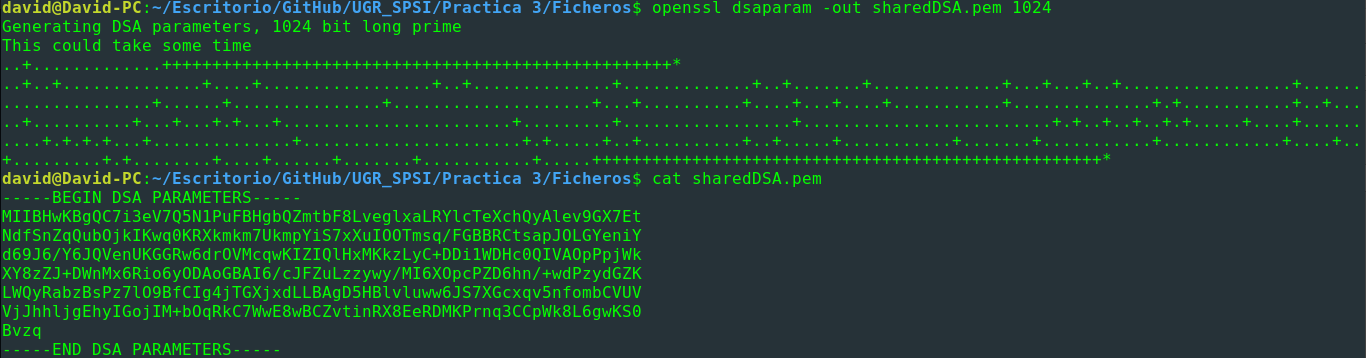
\includegraphics[width=1\textwidth]{./Imagenes/1.png}
\end{figure}


% ----------------------------------------------------------------
\chapter{Ejercicio 2}

\section{Enunciado}
\noindent
Generad dos parejas de claves para los parámetros anteriores. Las claves se almacenarán en los archivos nombreDSAkey.pem y apellidoDSAkey.pem. No es necesario protegerlas por contraseña.

\section{Respuesta}
\noindent
Para generar las dos parejas de claves utilizando los parámetros generados en el ejercicio anterior utilizamos el comando gendsa pasandole como entrada el archivo sharedDSA.pem como se muestra en la siguiente imagen.

\begin{figure}[!hbp]
 \centering  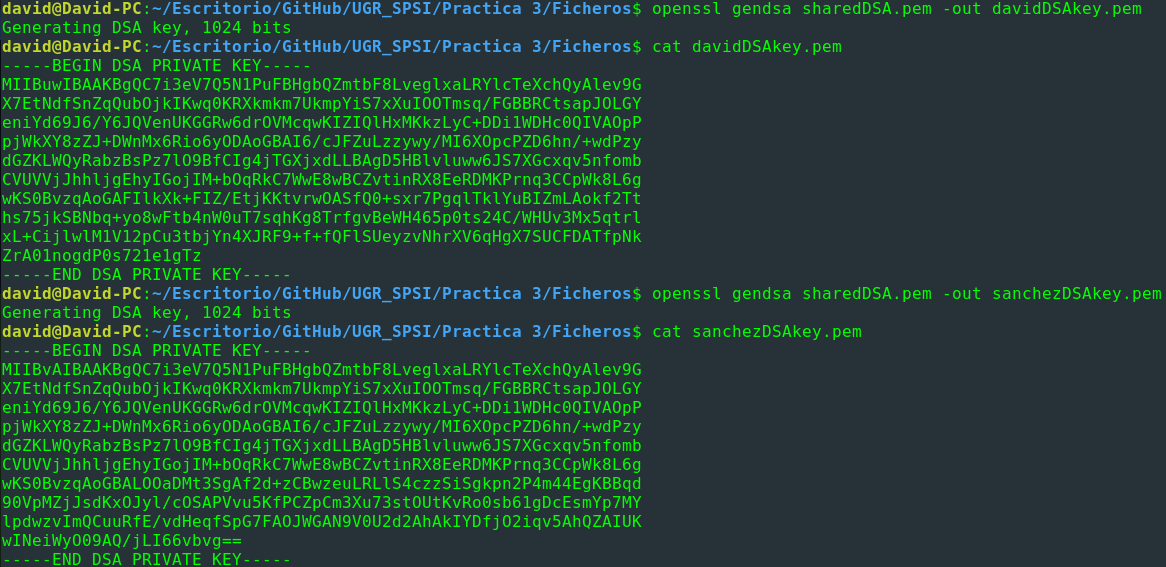
\includegraphics[width=1\textwidth]{./Imagenes/2.png}
\end{figure}

\noindent
Podemos observar similitudes en las siete primeras lineas de davidDSAkey.pem y sanchezDSAkey.pem.

% ----------------------------------------------------------------
\chapter{Ejercicio 3}

\section{Enunciado}
\noindent
Extraed la clave privada contenida en el archivo nombreDSAkey.pem a otro archivo que tenga por nombre nombreDSApriv.pem. Este archivo deberá estar protegido por contraseña. Mostrad sus valores. Lo mismo para el archivo apellidoDSAkey.pem.

\section{Respuesta}
\noindent
Para extraer la clave privada contenida en el archivo davidDSAkey.pem al archivo davidDSApriv.pem he utilizado cifrado aes 128. Como contraseña he utilizado 0123456789.

\begin{figure}[!hbp]
 \centering  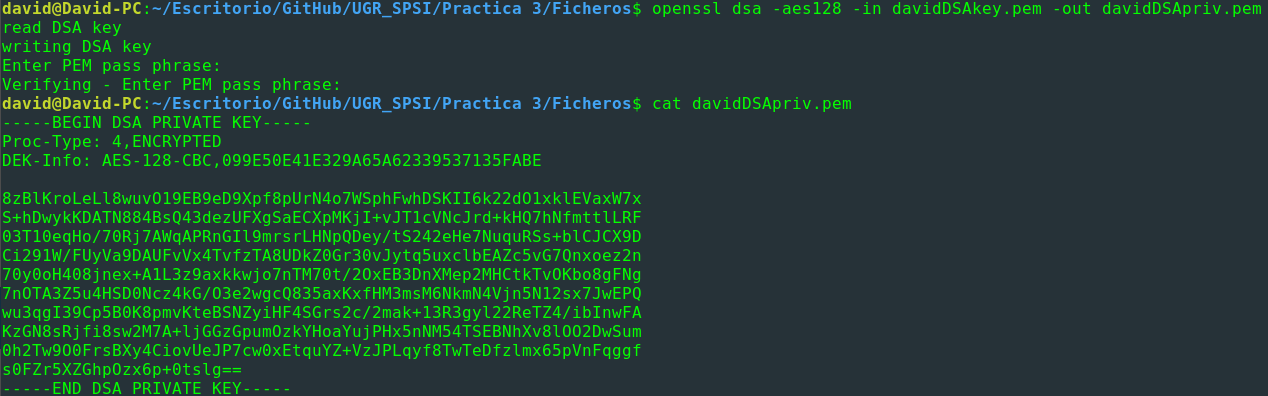
\includegraphics[width=1\textwidth]{./Imagenes/3_0.png}
\end{figure}

\noindent
Ahora paso a mostrar el fichero generado:
% \begin{figure}[!hbp]
%  \centering  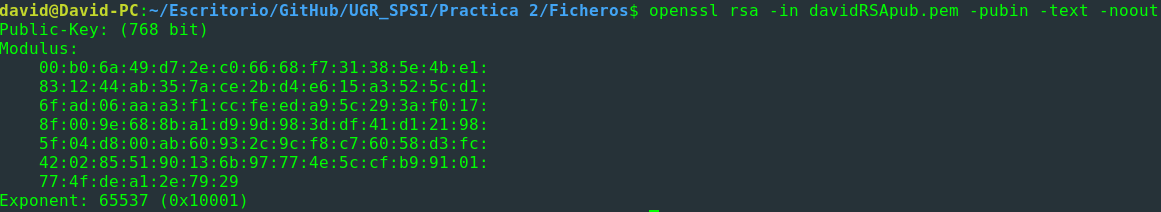
\includegraphics[width=1\textwidth]{./Imagenes/3_1.png}
% \end{figure}

\newpage
\noindent
Para la extraer la clave privada contenida en el archivo sanchezDSAkey.pem repito los mismos pasos:

\begin{figure}[!hbp]
 \centering  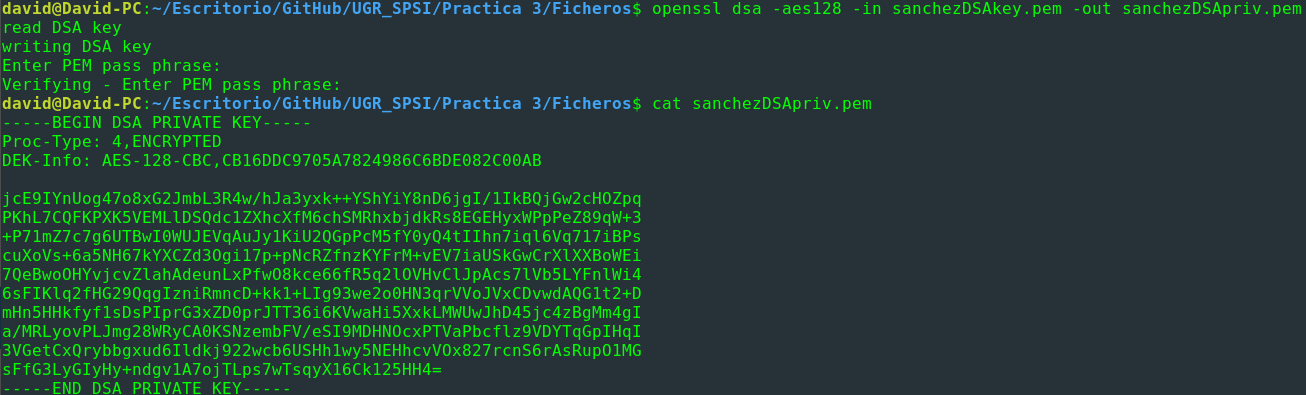
\includegraphics[width=1\textwidth]{./Imagenes/3_2.png}
\end{figure}

\noindent
Este es el contenido del archivo sanchezDSApriv.pem.

% \begin{figure}[!hbp]
%  \centering  \includegraphics[width=1\textwidth]{./Imagenes/3_3.png}
% \end{figure}

% ----------------------------------------------------------------
\chapter{Ejercicio 4}

\section{Enunciado}
\noindent
Extraed en nombreDSApub.pem la clave pública contenida en el archivo nombreDSAkey.pem. De nuevo nombreDSApub.pem no debe estar cifrado ni protegido. Mostrad sus valores. Lo mismo para el archivo apellidoDSAkey.pem

\section{Respuesta}
\noindent
Para extraer la clave pública contenida en davidDSAkey.pem en davidDSApub.pem utilizamos el modificador -pubout. Hacemos lo mismo con sanchezDSAkey.pem.
Estos son los valores de ambos archivos.

\begin{figure}[!hbp]
 \centering  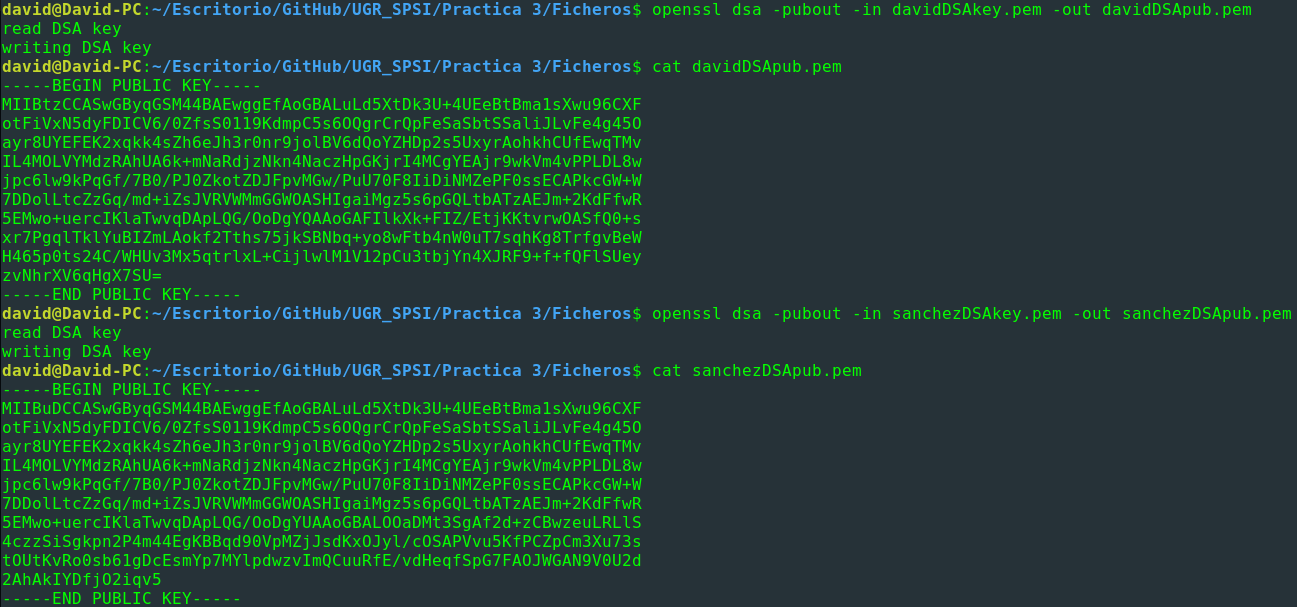
\includegraphics[width=1\textwidth]{./Imagenes/4.png}
\end{figure}

% ----------------------------------------------------------------
\chapter{Ejercicio 5}

\section{Enunciado}
\noindent
Calculad el valor hash del archivo con la clave pública nombreDSApub.pem usando sha384 con salida hexadecimal con bloques de dos caracteres separados por dos puntos. Mostrad los valores por salida estándar y guardadlo en nombreDSApub.sha384.

\section{Respuesta}
\noindent
Calculamos el valor hash del archivo davidDSApub.pem con openssl dgst usando sha384 y -hex para la salida exadecimal. Para que los bloques del codigo exadecimal sean de dos caracteres separados por : utilizamos el modificador -c. Por último redireccionamos la salida al archivo davidDSApub.sha384 para guardar la salida de el comando dentro de este archivo. Finalmente muestro el contenido del archivo.

\begin{figure}[!hbp]
 \centering  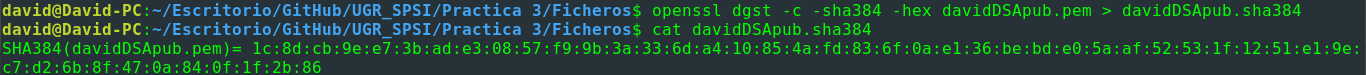
\includegraphics[width=1\textwidth]{./Imagenes/5.png}
\end{figure}

% ----------------------------------------------------------------
\chapter{Ejercicio 6}

\section{Enunciado}
\noindent
Calculad el valor hash del archivo con la clave pública apellidoDSApub.pem usando una función hash de 160 bits con salida binaria. Guardad el hash en apellidoDSApub.[algoritmo] y mostrad su contenido.

\section{Respuesta}
\noindent
Calculamos el valor hash del archivo sanchezDSApub.pem con openssl dgst usando la funcion hash sha1 que es de 160 bits. Utilizamos -binary para que la salida sea en binario. Redireccionamos la salida al archivo sanchezDSApub.sha1 para guardar la salida de el comando dentro de este archivo. Finalmente muestro el contenido del archivo utilizando xxd.

\begin{figure}[!hbp]
 \centering  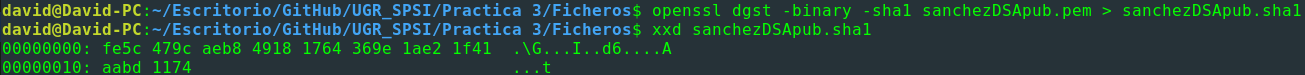
\includegraphics[width=1\textwidth]{./Imagenes/6.png}
\end{figure}


% ----------------------------------------------------------------
\chapter{Ejercicio 7}

\section{Enunciado}
\noindent
Generad el valor HMAC del archivo sharedDSA.pem con clave '12345' mostrándolo por pantalla.

\section{Respuesta}
\noindent
Para generar el valor HMAC del archivo sharedDSA.pem utilizo -hmac y la clave 12345 con el comando dgst como muestro en la siguiente imagen.

\begin{figure}[!hbp]
 \centering  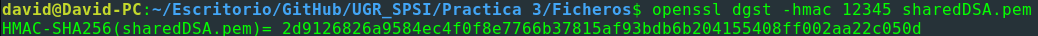
\includegraphics[width=1\textwidth]{./Imagenes/7.png}
\end{figure}


% ----------------------------------------------------------------
\chapter{Ejercicio 8}

\section{Enunciado}
\noindent
Simulad una ejecución completa del protocolo Estación a Estación. Para ello emplearemos como claves para firma/verificación las generadas en esta práctica, y para el protocolo DH emplearemos las claves asociadas a curvas elípticas de la práctica anterior junto con las de otro usuario simulado que deberéis generar nuevamente. Por otro ejemplo, si mi clave privada está en javierECpriv.pem y la clave pública del otro usuario está en lobilloECpub.pem, el comando para generar la clave derivada será:

\begin{lstlisting}[language=bash]
$> openssl pkeyutl -inkey javierECpriv.pem -peerkey
   lobilloECpub.pem -derive -out key.bin
\end{lstlisting}

\noindent
El algoritmo simétrico a utilizar en el protocolo estación a estación será AES-128 en modo CFB8.


\section{Respuesta}
\noindent

\end{document}
